% Cross-Domain Reference-Free Quality Estimation for Sentence Segmentation
% Draft v1 (2026-11-21), written from paper/outline.md v5.4. All numbers are tie-exact and use the adopted scoring
% function (normalized Soft F1 with the document end counted); sources: results/a11, a12, a13, review_fixes.
% Build: needs acl.sty and acl_natbib.bst from https://github.com/acl-org/acl-style-files (or the ACL Overleaf
% template); figures from `.venv/bin/python paper/figures/make_figures.py`, appendix tables from
% `python3 paper/figures/make_tables.py`.

\documentclass[11pt]{article}
\usepackage[final]{acl}
\usepackage{times}
\usepackage{latexsym}
\usepackage[T1]{fontenc}
\usepackage[utf8]{inputenc}
\usepackage{microtype}
\usepackage{inconsolata}
\usepackage{graphicx}
\usepackage{booktabs}
\usepackage{amsmath}
\usepackage{amssymb}
\usepackage{xcolor}

\newcommand{\Qt}{\tilde{Q}}
\newcommand{\Fone}{\mathrm{F}_1}
\newcommand{\sig}{^{*}}
\newcommand{\stat}[1]{\textsc{#1}}
% shrink a table to the line width only if it is wider (never enlarges)
\newcommand{\fitbox}[1]{\resizebox{\ifdim\width>\linewidth\linewidth\else\width\fi}{!}{#1}}

\title{Cross-Domain Reference-Free Quality Estimation\\for Sentence Segmentation}

% TODO(team): full names, NetIDs, contribution statement (see end matter)
\author{Weifeng [surname] \\
  New York University \\
  \And
  Yanhan [surname] \\
  New York University}

\begin{document}
\maketitle

\begin{abstract}
Sentence segmentation quality is hard to measure in a new domain, where gold boundaries are missing.
Reference-free quality estimation for segmentation has received little attention, and so has the question of how to
evaluate such an estimator. We build an evaluator that predicts a boundary probability at every gap between words,
fusing regular-expression rules, a Kneser--Ney $n$-gram model, a probe on a frozen BERT and two pretrained neural
boundary models, and that scores a segmentation by its normalized Soft F1 against these probabilities. We evaluate it on
the outputs of Punkt, Stanza, WtP and SaT on held-out English splits, against simple and adapted baselines, with three
views: agreement with true quality, agreement on the ranking of segmenters, and controlled error injection with a
quality-neutral control. On a fresh split of web text the evaluator reaches a Spearman correlation of 0.80 with true
quality (0.85 when paragraph structure is given), well above heuristics, language-model perplexity and system consensus
(0.66), and comparable to a strong supervised segmenter used as an evaluator. Error injection shows what remains hard:
boundaries without terminal punctuation, false splits after abbreviations, and annotation conventions that differ from
the training corpus.
\end{abstract}

% =====================================================================================================================
\section{Introduction}
\label{sec:intro}

Sentence segmentation is the first step of most NLP pipelines, and its errors propagate into parsing, translation and
retrieval. Segmenters differ in how they work---unsupervised abbreviation statistics in Punkt
\citep{kiss-strunk-2006-unsupervised}, supervised taggers trained on treebanks in Stanza \citep{qi-etal-2020-stanza},
punctuation-agnostic transformers in WtP and SaT \citep{minixhofer-etal-2023-wheres,frohmann-etal-2024-segment}---and
they behave differently across domains \citep{read-etal-2012-sentence}. A segmenter that is nearly perfect on news can
fail on forum posts without punctuation, on headlines or on lists. Yet whoever applies a segmenter to a new domain
usually has no gold boundaries with which to check its output.

We study \emph{reference-free quality estimation} for sentence segmentation: given raw text and a segmenter's output,
estimate the output's quality without gold boundaries for the target domain. This is a different task from
\emph{splitting}. A splitter must produce boundaries; a quality estimator judges an existing segmentation and can be used
to compare segmenters, to flag badly segmented documents, or to choose a segmenter for a new domain. Gold boundaries of a
source corpus (here GUM) may be used for training; target-domain gold is used only to validate the estimator.
Reference-based metrics---boundary precision, recall and F1, $P_k$, WindowDiff---cannot be computed in this setting.
Reference-free quality estimation is established for machine translation \citep{specia-etal-2018-quality}, but it is
underexplored for segmentation, so we also have to answer a second question: \emph{how should such an estimator be
evaluated?}

Our evaluator (Figure~\ref{fig:overview}) has two parts. It first predicts a boundary probability $p_i$ at every gap
between words, fusing techniques from the course \citep{jurafsky-martin-slp3}---regular-expression rules, a Kneser--Ney $n$-gram
model, a maximum-entropy probe---with pretrained neural boundary models; the fusion is trained on GUM so that the resulting scores
track true quality. It then scores a candidate segmentation by its \emph{normalized Soft F1} against these
probabilities, a score that is comparable across documents and well defined for documents with a single sentence. We ask:

\begin{itemize}
  \setlength\itemsep{0pt}
  \item[\textbf{RQ1}] Can a reference-free score rank real segmentation outputs by their true quality on held-out data,
  and how does it compare with the evaluators a practitioner would naturally try? (\S\ref{sec:rq1})
  \item[\textbf{RQ2}] Which segmentation errors does it notice, and what limits its reliability?
  (\S\ref{sec:rq2a}--\ref{sec:rq2b})
\end{itemize}

\noindent Our contributions are:
\begin{enumerate}
  \setlength\itemsep{0pt}
  \item \textbf{Method} (\S\ref{sec:method}): a reference-free quality estimator for sentence segmentation that fuses
  probabilistic boundary evidence---rules, a Kneser--Ney trigram model, a maximum-entropy probe on frozen BERT, zero-shot
  SaT and a fine-tuned boundary tagger---and scores an existing segmentation by normalized Soft F1 with a document-end
  correction.
  \item \textbf{Evaluation design} (\S\ref{sec:eval}): three views---agreement with true quality, the ranking of
  segmenters, and sensitivity to specific error types with a quality-neutral control---against nine baselines (rules,
  language models, a strong segmenter used as pseudo-reference or as evidence, multi-system consensus); gold isolation and
  pre-registered one-shot tests of the final evaluator on new held-out splits.
  \item \textbf{Findings} (\S\ref{sec:results}): on the fresh EWT dev split the evaluator reaches Spearman $\rho = 0.797$,
  $+0.141$ [$+0.075$, $+0.213$] over system consensus (0.851 given paragraph structure), on par with the strongest
  supervised segmenter plugged into the same scoring ($+0.035$, n.s.). Error injection shows complementary blind spots
  and the limits of transfer across annotation conventions.
\end{enumerate}

\begin{figure*}[t]
  \centering
  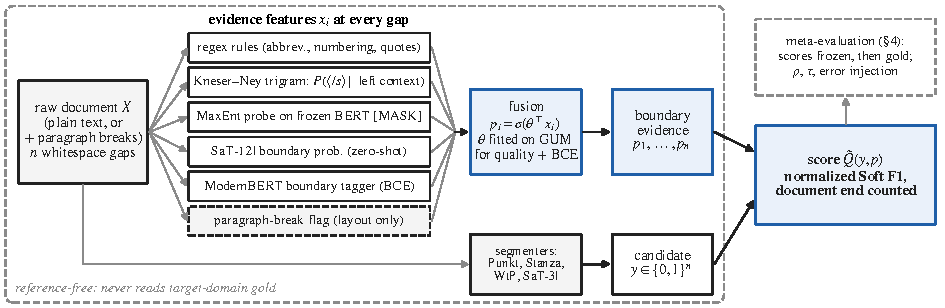
\includegraphics[width=\textwidth]{figures/f1_overview.pdf}
  \caption{The evaluator. Every source of evidence reads only the raw document; their features are fused into a
  boundary probability $p_i$ per gap, and each candidate segmentation is scored against $p$ by normalized Soft F1
  (\S\ref{sec:scoring}). Gold of the evaluated corpus is read only after all scores are frozen (\S\ref{sec:protocol}).
  The paragraph-break flag is used only in the controlled ``paragraphs given'' condition (\S\ref{sec:data}).}
  \label{fig:overview}
\end{figure*}

% =====================================================================================================================
\section{Related Work}
\label{sec:related}

\paragraph{Sentence segmentation.} Early work cast sentence boundary detection as classifying punctuation marks, with
maximum-entropy \citep{reynar-ratnaparkhi-1997-maximum} or neural \citep{palmer-hearst-1997-adaptive} classifiers;
Punkt \citep{kiss-strunk-2006-unsupervised} learns abbreviations without supervision, and abbreviations remain a main
source of errors \citep{gillick-2009-sentence}. Stanza \citep{qi-etal-2020-stanza} segments jointly with tokenization,
trained on Universal Dependencies (UD) treebanks \citep{demarneffe-etal-2021-universal}. WtP and SaT
\citep{minixhofer-etal-2023-wheres,frohmann-etal-2024-segment} predict newline positions with transformers and are robust
to missing punctuation. \citet{read-etal-2012-sentence} show that accuracy varies strongly across genres and annotation
conventions---the variation we want to measure without gold.

\paragraph{Evaluation without references.} Segmentations are normally compared with a reference by boundary
P/R/F1, $P_k$ \citep{beeferman-etal-1999-statistical}, WindowDiff \citep{pevzner-hearst-2002-critique} or boundary edit
distance \citep{fournier-2013-evaluating}. Reference-free quality estimation is established for machine translation
\citep{specia-etal-2018-quality,rei-etal-2020-comet}, where a metric is judged by its correlation with human judgments
\citep{freitag-etal-2021-results}. Without references, outputs of other systems can act as pseudo-references
\citep{albrecht-hwa-2007-regression,louis-nenkova-2013-automatically,gao-etal-2020-supert}, and noisy votes can be
aggregated by Dawid--Skene EM \citep{dawid-skene-1979-maximum}; both serve as baselines here.

\paragraph{Testing evaluators.} Correlation can hide what a metric cannot see. Behavioral tests
\citep{ribeiro-etal-2020-beyond} and perturbation checklists for generation metrics \citep{sai-etal-2021-perturbation}
inject controlled errors, and \citet{deutsch-etal-2022-limitations} show that reference-free metrics favor outputs that
resemble their own underlying models. We use both ideas: error injection with a quality-neutral control
(\S\ref{sec:views}) and a check for same-family bias (\S\ref{sec:rq1}). We are not aware of work that evaluates
reference-free estimators of sentence segmentation quality in this way.

% =====================================================================================================================
\section{Method}
\label{sec:method}

\subsection{Task}
\label{sec:task}
A document $X$ has words $w_1,\dots,w_{n+1}$ separated by whitespace; gap $i$ follows $w_i$. A segmentation is a vector
$y \in \{0,1\}^n$, where $y_i = 1$ means that a sentence ends after $w_i$; the end of the document is always a boundary
and is not part of $y$. With gold boundaries $g$, the true quality of $y$ is the boundary F1
\begin{equation}
  \Fone(y, g) = \frac{2\, y^{\top} g}{|y| + |g|} \qquad (\Fone = 1 \text{ if } |y| = |g| = 0),
  \label{eq:f1}
\end{equation}
with $|y| = \sum_i y_i$. An evaluator assigns a score $s(X, y)$ without reading the gold of the evaluated corpus. It is
useful to the extent that it orders candidates---within a document and across documents---as $\Fone$ does.

\subsection{Scoring a candidate against soft evidence}
\label{sec:scoring}
Suppose an evidence model gives a boundary probability $p_i \in [0,1]$ at every gap (\S\ref{sec:evidence}). We score $y$
by its F1 against $p$ used as a soft reference, counting the final boundary of the document, which every candidate and
the evidence get right, and normalize by the best score any candidate can reach:
\begin{gather}
  Q(y, p) = \frac{2\,(y^{\top} p + 1)}{|y| + \textstyle\sum_i p_i + 2}, \label{eq:q}\\
  \Qt(y, p) = \frac{Q(y, p)}{\max_{y'} Q(y', p)}, \quad
  \max_{y'} Q(y',p) = \max_{k=0,\dots,n} \frac{2\,(S_k + 1)}{k + \sum_i p_i + 2}, \label{eq:qnorm}
\end{gather}
where $S_k$ is the sum of the $k$ largest $p_i$: for a fixed number $k$ of cuts, $Q$ is largest when the cuts are at the
$k$ most probable gaps, so the maximum over all $2^n$ candidates needs only a sort. Three properties make this the right
score for our purpose.
\emph{(i) Local rewards.} Adding a cut at gap $i$ raises $Q$ exactly when $p_i > Q/2$, so a candidate is rewarded for
cutting where the evidence is confident and penalized elsewhere.
\emph{(ii) Comparability across documents.} How high a candidate can score depends on how peaked $p$ is in its document;
dividing by the attainable maximum makes $\Qt = 1$ mean ``as good as the evidence allows'' in every document. This
matters for our primary criterion, which pools candidates from all documents (\S\ref{sec:views}).
\emph{(iii) Single-sentence documents.} Without the $+1$ terms, the correct empty segmentation of a one-sentence document
has Soft F1 $= 0$ for every $p$ and is ranked last. With them it scores $2/(\sum_i p_i + 2)$ before normalization, and
$\Qt$ is close to 1 when the evidence puts little mass inside the document (e.g., $\Qt = 0.95$ when two internal gaps
have $p = 0.4$). Figure~\ref{fig:example} shows the computation on a real document.

\begin{figure}[t]
  \centering
  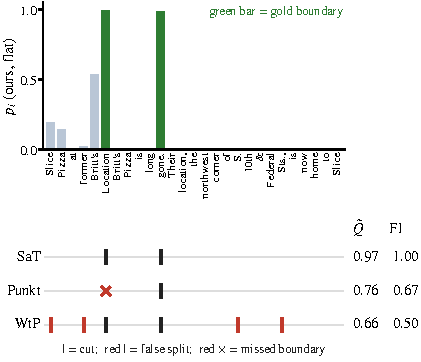
\includegraphics[width=\columnwidth]{figures/f2_example.pdf}
  \caption{A worked example: an EWT dev review whose first ``sentence'' is a title without punctuation. Bars: our flat
  evaluator's $p_i$ at each gap (labeled by the word before it). Rows: three real segmenter outputs. Punkt misses the
  unpunctuated title boundary; WtP adds false splits, two of them after the abbreviations \emph{S.} and \emph{Sts.,}.
  $\Qt$ orders the three candidates as true F1 does. Gold scores 0.97 rather than 1 because the evidence also puts
  $p = 0.54$ before the capitalized word \emph{Location}.}
  \label{fig:example}
\end{figure}

\subsection{Boundary evidence}
\label{sec:evidence}
Table~\ref{tab:evidence} lists the sources of evidence. Each produces features at every gap from the raw text alone.
The maximum-entropy probe places a \texttt{[MASK]} token at gap $i$ in a frozen \texttt{bert-base-uncased}
\citep{devlin-etal-2019-bert}---replacing a visible \emph{.?!} before the gap, inserting it otherwise---and classifies the
hidden states:
\begin{equation}
  p^{\text{probe}}_i = \sigma\big(w^{\top} [\,h^{(8)}_i;\, h^{(12)}_i;\, \ell_i\,] + b\big),
  \label{eq:probe}
\end{equation}
where $h^{(l)}_i$ is the layer-$l$ state at the mask and $\ell_i$ are insertion likelihood ratios (how much the masked
log-probabilities of the neighboring tokens change when a period is inserted). The probe is an L2-regularized logistic
regression \citep{alain-bengio-2016-understanding}. The two pretrained neural sources are the boundary probability of
SaT-12l \citep{frohmann-etal-2024-segment}, used zero-shot, and a ModernBERT-large encoder
\citep{warner-etal-2024-modernbert} that we fine-tune on GUM as a binary boundary tagger (one logit per word, binary
cross-entropy). All sources read lower-cased text except SaT-12l, which reads the original casing in the flat evaluator.

\begin{table}[t]
  \centering
  \small
  \setlength{\tabcolsep}{3pt}
  \fitbox{\begin{tabular}{@{}p{2.25cm}p{3.15cm}p{1.35cm}@{}}
    \toprule
    Source & Captures & Course topic \\
    \midrule
    Regex rules (24) & abbreviations, initials, numbering, times, quotes, distance to punctuation & regular expressions \\
    Kneser--Ney trigram (4) & $\log P(\langle/s\rangle \mid$ two left words$)$, start / continuation probabilities &
      $n$-gram LMs \\
    Probe on BERT (1) & Eq.~\ref{eq:probe}: punctuation vs.\ sentence boundary in context & MaxEnt / logistic reg. \\
    SaT-12l (1) & pretrained boundary model, zero-shot & --- \\
    ModernBERT tagger (1) & boundary tagger fine-tuned on GUM & sequence labeling \\
    Paragraph flag (1) & newline at the gap (layout only) & --- \\
    \bottomrule
  \end{tabular}}
  \caption{Evidence sources (number of features in parentheses). Rules and $n$-gram counts are fitted on GUM train only;
  details in App.~\ref{app:method}.}
  \label{tab:evidence}
\end{table}

\subsection{Fusion trained for quality}
\label{sec:fusion}
The features of gap $i$ are stacked into $x_i$ (31 dimensions; 32 with the paragraph flag) and fused by a logistic model
$p_i = \sigma(\theta^{\top} x_i)$. A plain boundary classifier treats all gaps alike, although most gaps are easy and only
the few where segmenters disagree decide which candidate is better. We therefore fit $\theta$ on GUM train for both
boundary accuracy and score quality:
\begin{gather}
  J(\theta) = \frac{L_Q(\theta)}{L_Q(\theta_0)} + \frac{L_B(\theta) + \frac{\lambda}{2}\lVert\theta\rVert^2}{L_B(\theta_0)},
  \label{eq:objective}\\
  L_Q(\theta) = \frac{1}{|\mathcal{I}|}\sum_{(d,s)\in\mathcal{I}} \big(\Qt^{0}(y_{ds}, p_\theta) - \Fone(y_{ds}, g_d)\big)^2,
  \nonumber
\end{gather}
where $\mathcal{I}$ contains every training document $d$ paired with the output $y_{ds}$ of each of the four segmenters
$s$, $L_B$ is the mean binary cross-entropy of $p_\theta$ against gold over all gaps, and $\theta_0$ is the
boundary-only solution (L2 logistic regression, $\lambda = 10^{-3}$), which also initializes L-BFGS
\citep{liu-nocedal-1989-limited}; gradients pass through the sort in Eq.~\ref{eq:qnorm}. As implemented, the training
objective uses the normalized Soft F1 \emph{without} the document-end term ($\Qt^0$), while evaluation uses $\Qt$. No GUM
document is a single sentence; there the two scores differ per item by 0.001--0.002 on average (at most 0.04) and give the
same agreement with true quality to three decimals (0.903 flat, 0.948 with paragraphs), so we kept the frozen models.
In a controlled comparison on GUM (same features, folds and items), this objective beats boundary-only training, whereas
a quality loss alone or a post-hoc quality-estimation regression over the four seen segmenters does not, and both
degrade when a segmenter is held out (App.~\ref{app:objective}).

We fit two evaluators: \emph{flat}, for plain text (the default), and \emph{layout}, which also sees paragraph breaks
(\S\ref{sec:data}); the layout evaluator is lower-cased throughout and adds the paragraph flag.

\subsection{What we tried on the way}
\label{sec:tried}
Our first evaluators used the Platt-calibrated BERT probability of a terminal punctuation mark at the gap
(\emph{PuncEv}), and then the probe alone; each was frozen and tested once on EWT test. A semi-Markov sentence-length
prior on top of the evidence did not help on any corpus; letting BERT see the candidate's own boundaries made the
evidence agree with the candidate's errors; post-hoc quality regression learned the four seen segmenters rather than
quality; and a left-to-right LLM (Qwen) gave evidence that normalization could not make comparable across documents.
App.~\ref{app:prelim}--\ref{app:method} give details; the development ladder from the probe to the final evaluator is in
App.~\ref{app:ladder}.

% =====================================================================================================================
\section{Evaluating an Evaluator}
\label{sec:eval}

\subsection{Data, segmenters and input conditions}
\label{sec:data}
Table~\ref{tab:data} lists the corpora, all English UD treebanks. GUM train \citep{zeldes-2017-gum} is used for training
and development by leave-one-genre-out cross-fitting (15 genres). EWT test \citep{silveira-etal-2014-gold}, GENTLE
test \citep{aoyama-etal-2023-gentle} and LinES test \citep{ahrenberg-2007-lines} were used to test earlier frozen
versions of the evaluator, so their numbers for the final evaluator are \emph{re-used} tests (R). EWT dev and LinES
train+dev had never been processed before the final evaluator's one-shot test (T); they are new documents, not new
domains. GUM test is never read. The candidates are the outputs of Punkt, Stanza, WtP (\texttt{wtp-bert-mini}) and SaT
(\texttt{sat-3l-sm}) with default settings; an \emph{item} is a document paired with one segmenter's output. Training-data
overlap: Stanza's English model was trained on GUM and EWT training data and the SaT-sm models on UD training data
including GUM train; the test splits of GENTLE and LinES are unseen by all models.

\begin{table}[t]
  \centering
  \small
  \setlength{\tabcolsep}{3.2pt}
  \fitbox{\begin{tabular}{@{}lrrrrrc@{}}
    \toprule
    Split & Docs & Gen. & Words & Bound. & No punct. & Status \\
    \midrule
    GUM train & 197 & 15 & 169k & 11{,}117 & 10.9\% & D \\
    GENTLE test & 26 & 8 & 15k & 1{,}308 & 43.1\% & R \\
    LinES test & 9 & -- & 17k & 1{,}112 & 6.2\% & R \\
    EWT test & 316 & 5 & 22k & 1{,}761 & 29.8\% & R \\
    EWT dev & 318 & 5 & 22k & 1{,}683 & 23.9\% & T \\
    LinES tr+dev & 18 & -- & 75k & 4{,}557 & 6.3\% & T \\
    \bottomrule
  \end{tabular}}
  \caption{Corpora. Bound.: gold sentence boundaries inside documents; No punct.: share of them whose preceding word does
  not end in terminal punctuation (titles, list items, dashes, missing periods). EWT test and dev contain 33 and 42
  single-sentence documents. Status of the final evaluator's numbers: D development (leave-one-genre-out), R re-used test,
  T pre-registered one-shot test. LinES has no genre labels and is resampled as one stratum.}
  \label{tab:data}
\end{table}

\paragraph{Input conditions.} \emph{Flat text} is the default, fully reference-free setting: paragraph breaks are
replaced by spaces. \emph{Paragraph layout} is a controlled condition in which the paragraph breaks recorded in UD
(\texttt{\# newpar}) are given as newlines to segmenters and evaluators. In UD every paragraph break is a sentence
boundary, so this condition supplies part of the gold structure; we report it as ``paragraphs given'', not as raw text.
LinES has no paragraph markup and appears only in the flat condition.

\subsection{Baselines}
\label{sec:baselines}
We compare with the evaluators a reader would naturally try. \textbf{B1} punctuation rule: candidate F1 against a
pseudo-reference that cuts after every terminal punctuation mark. \textbf{B2} length prior: mean log-probability of the
candidate's sentence lengths under the GUM length distribution. \textbf{B3} masked LM: the PuncEv probability of
\S\ref{sec:tried} with our scoring $\Qt$. \textbf{B4} the strongest available segmenter, SaT-12l-sm, as
pseudo-reference (candidate F1 against its segmentation). \textbf{B5} SaT-12l-sm's Platt-calibrated
\citep{platt-1999-probabilistic} boundary probabilities with our scoring $\Qt$. \textbf{B6} consensus: F1 against the
majority vote of the other three segmenters. \textbf{B7} DocAgree: the mean pairwise F1 among the four outputs, which
measures only how hard a document is (constant within a document). \textbf{B8} GPT-2 \citep{radford-etal-2019-language}
perplexity: mean token log-likelihood of the text written one sentence per line. \textbf{B9} Dawid--Skene EM over the four
segmenters' votes \citep{dawid-skene-1979-maximum}, leave-one-out posterior of the other three systems, with our scoring.
In the layout condition the baselines also see the paragraph breaks. All learned parts (B2, B5, B9) are fitted on GUM
or on the evaluated system outputs only. Note that SaT-12l-sm was trained on GUM train.

\subsection{Three views}
\label{sec:views}
\paragraph{V1: agreement with true quality.} Our primary criterion is the Spearman correlation over \emph{all} items
of a corpus,
\begin{equation}
  \rho = \operatorname{Spearman}\big(\{s(X_d, y_{ds})\},\ \{\Fone(y_{ds}, g_d)\}\big)_{(d,s)},
  \label{eq:rho}
\end{equation}
which requires scores to be comparable across documents and domains. We also report within-document pairwise accuracy:
the share of pairs of segmenters on the same document with different true F1 that the score orders correctly (score ties
count $\frac12$).

\paragraph{V2: ranking the segmenters.} Kendall's $\tau_b$ between the evaluator's ranking of the four segmenters (by mean
score) and their true ranking (by mean F1), computed per genre and averaged (and per document).

\paragraph{V3: controlled sensitivity.} For each document we take the gold segmentation $g$ and inject exactly one error
of a given type, 20 times at random positions. The \emph{detection rate} is the probability that the score drops,
\begin{equation}
  D_t = \Pr\big[s(X, g \oplus e_t) < s(X, g)\big] + \tfrac12 \Pr\big[s(X, g \oplus e_t) = s(X, g)\big],
  \label{eq:detection}
\end{equation}
averaged over documents that contain a position of type $t$. Error types: removing a gold boundary after terminal
punctuation (M-term), without terminal punctuation at a paragraph break (M-par) or inside a paragraph (M-inpar); adding a
false boundary after a period that does not end a sentence, i.e.\ after abbreviations or numbering (S-abbr), after other
punctuation such as a comma (S-punct), or with no punctuation (S-none); and shifting a boundary by up to three words. The
\emph{control} moves one injected false boundary to another random non-boundary gap, which leaves true quality
unchanged. Because the two positions are exchangeable, every evaluator sits at 0.5 in expectation; the control is a
sanity check of the procedure (no directional bias, correct handling of ties), not evidence that a response is driven by
quality. An error type counts as detected when the 95\% CI of $D_t$ lies above 0.5. V3 is needed because V1 can be high
without any sensitivity: DocAgree reacts to no error at all, yet reaches $\rho = 0.51$--$0.77$.

\subsection{Protocol and status of the numbers}
\label{sec:protocol}
Scores are written to disk before gold is loaded (gold isolation). All method decisions were made on GUM by
leave-one-genre-out cross-fitting, with selection rules written down before the results were computed; the
protocol was amended 13 times, always before the affected numbers existed (App.~\ref{app:protocol}). Confidence intervals
come from a genre-stratified document bootstrap \citep{efron-tibshirani-1993-introduction} with 1000 resamples; paired
differences use the same resamples. For the final evaluator, GUM numbers are development (D); GENTLE, LinES test and EWT
test are re-used tests (R); EWT dev and LinES train+dev are pre-registered one-shot tests (T), with the primary hypothesis
that the final evaluator beats consensus in the layout condition. \textbf{All baseline numbers, comparisons with
baselines and the sensitivity test are post hoc (P)}: computed after the one-shot test, without changing the final
evaluator; baselines are fixed or fitted on GUM only.\footnote{Scores are rounded to $10^{-10}$ before ranking so that
identical segmentations get identical ranks. On GUM, the fused model is fitted leave-one-genre-out but its learned base
features (probe, tagger, $n$-gram) are not nested; refitting the probe and $n$-gram features nested changes the final
evaluator's GUM $\rho$ by $+0.0005$ (flat) and $+0.0007$ (layout), both n.s., so the GUM numbers are not inflated
(App.~\ref{app:protocol}).}

% =====================================================================================================================
\section{Results}
\label{sec:results}

\subsection{RQ1: Does the score track true quality?}
\label{sec:rq1}

\begin{table*}[t]
  \centering
  \small
  \setlength{\tabcolsep}{5pt}
  \fitbox{\begin{tabular}{@{}lcccccc@{}}
    \toprule
    & \multicolumn{5}{c}{Flat text} & Paragraphs given \\
    \cmidrule(lr){2-6}\cmidrule(l){7-7}
    Evaluator & EWT dev & LinES tr+dev & GENTLE & EWT test & LinES test & EWT dev \\
    & (T) & (T) & (R) & (R) & (R) & (T) \\
    \midrule
    B1 punctuation rule & 0.378 & 0.296 & 0.383 & 0.369 & 0.437 & 0.796 \\
    B3 masked LM (PuncEv) & 0.464 & 0.440 & 0.542 & 0.508 & 0.758 & 0.698 \\
    B8 GPT-2 perplexity & 0.062 & 0.049 & 0.064 & 0.043 & $-$0.322 & 0.039 \\
    B6 consensus & 0.657 & 0.468 & 0.830 & 0.657 & 0.861 & 0.625 \\
    B9 Dawid--Skene & 0.615 & 0.480 & 0.838 & 0.655 & 0.859 & 0.609 \\
    B4 SaT-12l-sm as reference & 0.738 & \textbf{0.630} & 0.880 & 0.754 & \textbf{0.888} & 0.797 \\
    B5 SaT-12l-sm probabilities & 0.762 & \textbf{0.630} & 0.891 & 0.778 & 0.873 & 0.835 \\
    \textbf{Ours} & \textbf{0.797} & 0.563 & \textbf{0.907} & \textbf{0.787} & 0.873 & \textbf{0.851} \\
    \bottomrule
  \end{tabular}}
  \caption{V1: global Spearman $\rho$ between score and true F1 over all items (Eq.~\ref{eq:rho}). B3, B5 and B9 use our
  scoring $\Qt$ on their own probabilities; B4 and B6 compute F1 against a pseudo-reference. Status letters refer to
  our evaluator; all baseline rows are post hoc (P). B2 length prior and B7 DocAgree, GUM (D), and all CIs and paired
  differences are in App.~\ref{app:agreement}.}
  \label{tab:agreement}
\end{table*}

\begin{figure*}[t]
  \centering
  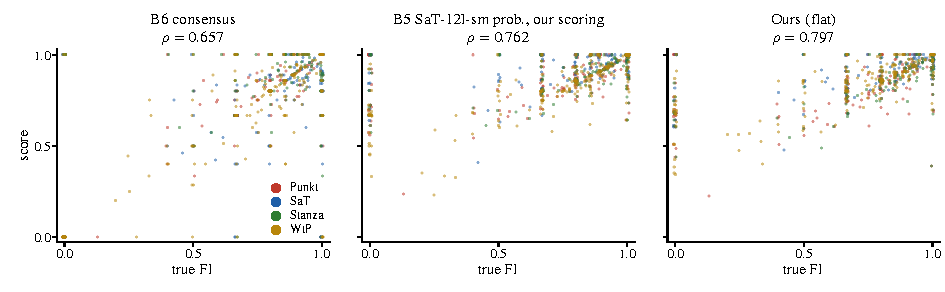
\includegraphics[width=\textwidth]{figures/f3_scatter.pdf}
  \caption{Score vs.\ true F1 for all 1{,}272 items of EWT dev (flat text, T for ours), colored by segmenter. Consensus
  takes few distinct values and gives full marks to many imperfect outputs. The column at true F1 $= 0$ (66 items) holds
  short documents in which a single boundary error drives F1 to 0, e.g., 32 single-sentence documents that a segmenter
  split; every evaluator scores many of them highly.}
  \label{fig:scatter}
\end{figure*}

Table~\ref{tab:agreement} and Figure~\ref{fig:scatter} show agreement with true quality. On the fresh EWT dev split our
evaluator reaches $\rho = 0.797$ on plain text. The paired differences (ours minus baseline, 95\% CI) are large against everything that
does not use a strong supervised segmenter: consensus $+0.141$ [$+0.075$, $+0.213$], Dawid--Skene $+0.183$ [$+0.117$,
$+0.253$], masked LM $+0.333$ [$+0.256$, $+0.414$], the punctuation rule $+0.419$ [$+0.334$, $+0.503$] and GPT-2
$+0.735$ [$+0.640$, $+0.838$]. Given paragraphs, our evaluator beats consensus by $+0.227$ [$+0.158$, $+0.298$]---the
pre-registered primary test---and the rule by $+0.055$ [$+0.033$, $+0.083$]; the rule becomes strong (0.796) once
paragraph breaks are given, because most unpunctuated boundaries in EWT are paragraph breaks. On GENTLE the gain over
consensus is $+0.077$ [$+0.021$, $+0.141$]. LinES is different: on train+dev ours beats consensus only narrowly ($+0.095$
[$+0.007$, $+0.210$]) and the masked LM not significantly ($+0.124$ [$-0.061$, $+0.369$]); on LinES test the gain over
consensus is $+0.011$ (n.s.). GPT-2 perplexity is a useful contrast: it separates candidates within a document (pairwise
accuracy 0.71 on EWT dev) but not across documents, because its likelihood mostly reflects what a document is about---the
confound that normalization removes from Soft F1.

\paragraph{Against a strong segmenter.} Our evaluator is not significantly different from SaT-12l-sm's probabilities in
our scoring on any held-out split: EWT dev $+0.035$ [$-0.014$, $+0.088$], GENTLE $+0.015$ [$-0.035$, $+0.064$], LinES
train+dev $-0.066$ [$-0.236$, $+0.095$], where SaT is ahead (0.630 vs.\ 0.563). It is better than SaT's own segmentation
used as a reference on web text (EWT dev $+0.060$ [$+0.008$, $+0.112$]) but not elsewhere. So evidence that combines
course techniques with pretrained models is statistically indistinguishable from the best supervised segmenter used as
an evaluator; we show next that the
two fail on different errors. An unweighted average of the two is best on web text (EWT dev 0.808, $+0.046$
[$+0.003$, $+0.092$] over B5) but not on LinES (App.~\ref{app:agreement}).

\paragraph{Ranking the segmenters (V2).} Given paragraphs, ours and B5 rank the four segmenters perfectly in every EWT dev
genre (genre-mean $\tau = 1.0$), whereas consensus does not (0.47): it rewards the segmenter that agrees with the
majority, not the one that is right. On flat text the genre-level ranking is noisy for all evaluators (five genres;
ours 0.53, B5 0.67, consensus 0.60), while the document-level $\tau$ favors ours (0.70 vs.\ 0.52 for consensus).
SaT-based evaluators slightly overrate the SaT candidate (rank residual $+0.02$ to $+0.03$), a mild form of the
same-family bias of \citet{deutsch-etal-2022-limitations} (App.~\ref{app:agreement}).

Spearman correlation tells how well a score tracks quality overall. Which errors does it actually notice?

\subsection{RQ2a: Which errors does each evaluator notice?}
\label{sec:rq2a}

\begin{table}[t]
  \centering
  \small
  \setlength{\tabcolsep}{2.6pt}
  \fitbox{\begin{tabular}{@{}lcccccc@{}}
    \toprule
    & \multicolumn{3}{c}{Missed boundary} & \multicolumn{2}{c}{False split} & \\
    \cmidrule(lr){2-4}\cmidrule(lr){5-6}
    Evaluator & term. & par. & in-par. & abbr. & punct. & Ctrl. \\
    \midrule
    B1 rule & 1.00\sig & 0.01 & 0.01 & 0.00 & 0.97\sig & 0.50 \\
    B8 GPT-2 & 0.82\sig & 0.86\sig & \textbf{0.89}\sig & 0.53 & 0.87\sig & 0.49 \\
    B6 consensus & 1.00\sig & 0.52 & 0.51 & 0.55 & 0.97\sig & 0.50 \\
    B5 SaT prob. & 0.96\sig & 0.85\sig & 0.64\sig & \textbf{0.75}\sig & 0.99\sig & 0.49 \\
    \textbf{Ours} (flat) & 0.99\sig & \textbf{0.93}\sig & 0.84\sig & 0.66\sig & 0.97\sig & 0.50 \\
    Ours (par.) & 0.99\sig & 1.00\sig & 0.31 & 0.69\sig & 1.00\sig & 0.49 \\
    \bottomrule
  \end{tabular}}
  \caption{V3 on EWT dev: detection rate of one injected error (Eq.~\ref{eq:detection}); $^{*}$ = 95\% CI above 0.5; the
  control should be 0.50. Missed boundary after terminal punctuation (term.), without it at a paragraph break (par.) or
  inside a paragraph (in-par.); false split after an abbreviation or numbering (abbr.) or after other punctuation
  (punct.). Ours (par.): paragraphs given. Documents with such a position: 260, 113, 60, 53, 173. All evaluators, error
  types and corpora in App.~\ref{app:sensitivity}.}
  \label{tab:sensitivity}
\end{table}

Table~\ref{tab:sensitivity} shows the controlled test on EWT dev. The control sits at 0.50 for every evaluator, as the
procedure requires. Errors marked by punctuation---a missed boundary after a period, a false split after a comma---are
noticed by every evaluator that reads the text. Two error types separate the evaluators:

\paragraph{Missed boundaries without terminal punctuation.} The rule ignores them entirely (0.01). Consensus is at chance
(0.52 and 0.51), and Dawid--Skene barely above it (0.63 and 0.57): aggregating segmenters cannot reveal an error that most
of them make. Ours (flat) and GPT-2 are the most sensitive (0.84--0.93). The length prior is one-sided: it catches every
merge and no split (App.~\ref{app:sensitivity}).

\paragraph{False splits after abbreviations and numbering.} SaT-12l-sm probabilities are the most sensitive (0.75),
ours less so (0.66), and GPT-2 is at chance (0.53). The two strongest evaluators thus have \emph{complementary blind
spots}, which explains why their average helps (\S\ref{sec:rq1}).

\paragraph{Paragraph cues move the blind spot.} Given paragraph breaks, our evaluator catches every missed boundary at a
paragraph break (1.00) but misses most inside paragraphs (0.31): during training it learned that an unpunctuated boundary
is almost always a newline. The same happens on GUM (0.07) and GENTLE (0.17), and explains why the layout evaluator
should not be applied to text without layout (App.~\ref{app:blindspots}).

What, then, determines how reliable an evaluator is?

\subsection{RQ2b: What limits reliability?}
\label{sec:rq2b}

\paragraph{The scoring formula matters in two places.} Normalization across documents raises agreement on GUM by
$+0.24$ for PuncEv and $+0.05$ for ours (App.~\ref{app:agreement}); GPT-2 (\S\ref{sec:rq1}) shows what happens
without it. Counting the document end matters wherever single-sentence documents occur: on EWT dev it raises the final
evaluator's $\rho$ from 0.503 to 0.851 ($+0.348$ [$+0.251$, $+0.449$], T, with paragraphs; $+0.330$ flat). With both in
place, soft versus hard scoring of the \emph{same} probabilities matters little for our evidence (EWT dev $+0.005$ flat,
$+0.013$ with paragraphs) and helps SaT probabilities on web text ($+0.025$ [$+0.002$, $+0.053$] flat; n.s.\ on GENTLE
and LinES), in a controlled comparison with the same calibration and document-end convention
(App.~\ref{app:agreement}).

\paragraph{Then mostly the evidence.} Along our development each evidence component added agreement (GUM, flat: probe
0.57 $\to$ stack 0.82 $\to$ cased SaT 0.88 $\to$ quality training 0.90; on EWT dev 0.60 $\to$ 0.80;
App.~\ref{app:ladder}). Our evidence is comparable to the best supervised segmenter's probabilities, and neither covers
both hard error types (Table~\ref{tab:sensitivity}).

\paragraph{Consensus measures difficulty, not quality.} Consensus is good at telling \emph{which document is hard}
(between-document $\rho = 0.92$ on EWT dev with paragraphs, ours 0.88) and poor at telling \emph{which segmentation is
better} (within-document $\rho = 0.54$, ours 0.80).

\paragraph{Annotation conventions set the ceiling.} On LinES (both splits) all evaluators fall to $\rho \le 0.63$, and
false splits after abbreviations are detected at only 0.20--0.39 (App.~\ref{app:sensitivity}). LinES follows
different conventions from GUM: where LinES marks no boundary after terminal punctuation, GUM-trained evidence still
predicts one (mean $p = 0.77$ vs.\ 0.26 on GUM for the fused stack), so it cannot see false splits there, and the
improvements we developed on GUM do not transfer: the final evaluator is not better than the probe alone there
(pre-registered H5 failed, $-0.088$ [$-0.245$, $+0.075$]).

\paragraph{Selection.} The original motivation was to pick the best segmenter per domain. SaT-3l-sm is the best of the
four segmenters on every corpus (sometimes narrowly), and no evaluator selects better than always using it
(App.~\ref{app:selection}); ranking ability does not turn into a selection gain without headroom.

In short: once scores are normalized and the document end is counted, an evaluator is only as reliable as its evidence on
the few gaps that separate the candidates, and adding cues moves its blind spots rather than removing them.

% =====================================================================================================================
\section{Discussion}
\label{sec:discussion}

\paragraph{Main findings.} (1)~Reference-free quality estimation for sentence segmentation is feasible: with good
boundary evidence and a normalized, document-end-aware score, it tracks true quality on held-out splits and ranks
segmenters correctly. (2)~Evidence that fuses course techniques with pretrained neural models is comparable to a strong
off-the-shelf segmenter used as an evaluator; the two fail on different error types, and their unweighted average helps
on web text. (3)~Controlled error injection is needed next to correlation: it shows what each evaluator cannot see---
consensus misses shared errors, perplexity is not comparable across documents and ignores abbreviation errors, and
evidence trained with paragraph cues misses in-paragraph boundaries. Thresholded at 0.5, the boundary-only version
of our fused evidence is also a competitive segmenter in its own right, matching or beating the SaT system we evaluate
(App.~\ref{app:sat}).

\paragraph{Future work.} Better evidence for unpunctuated boundaries in text without layout; adapting the evidence to a
target corpus's annotation conventions from a handful of examples; combining evidence sources whose blind spots differ;
one objective for training and evaluation; and domains where the best segmenter changes, so that selection has room to
help.

% =====================================================================================================================
\section{Conclusion}
\label{sec:conclusion}
We built and evaluated a reference-free quality estimator for sentence segmentation. On held-out splits it tracks true
quality far better than heuristics, language-model perplexity or system consensus and is comparable to a strong
supervised segmenter used as an evaluator, while controlled error injection shows which errors it misses and why
differing annotation conventions limit its transfer.

\section*{Limitations}
English only, four segmenters and UD annotation. The layout condition takes paragraph breaks from UD, where they are
sentence boundaries by construction, so results with paragraphs are optimistic (``structure given''). The held-out sets are
small (GENTLE 26 documents, LinES 9 and 18) and the new splits are new documents, not new domains. Baseline comparisons
and the sensitivity test are post hoc; only the final evaluator's scores on EWT dev and LinES train+dev are one-shot tests,
and its numbers on GENTLE, LinES test and EWT test are re-used tests. The training objective omits the document-end term
used in evaluation (harmless on GUM, but not unified). Training data overlap: SaT-sm and Stanza were trained on GUM (and
Stanza on EWT); our evidence and SaT-12l-sm are both supervised on GUM, and GENTLE follows GUM's conventions. The design
was adaptive (13 dated, pre-registered amendments); the document-end correction was found post hoc on a re-used test and
then confirmed on a new split. An independent code review found five issues that affected reported numbers; after the
fixes, the pre-registered selections and all one-shot hypotheses are unchanged (App.~\ref{app:protocol}). Selecting a
segmenter was not shown to beat always using SaT, and transfer to different annotation conventions (LinES) fails.

\section*{Contributions and Availability}
% TODO(team): confirm the team-size / contribution statement with the instructor.
Weifeng: method, experiments, analysis, \S3--5 and appendix. Yanhan: \S1--2, figures, examples, presentation. Both:
\S6--7. Code, configurations, Slurm scripts and all result files are in the project repository; every number in this
paper is produced by a script listed in App.~\ref{app:protocol}.

\bibliography{references}

% =====================================================================================================================
\appendix
\onecolumn

\section{Preliminary Exploration}
\label{app:prelim}
Before real segmenter outputs were available, we studied synthetic candidates on GUM dev: gold-derived benchmarks in which
sentence-final punctuation was removed and Gold/Over/Under/Shift/Mixed candidates were generated, scored with the
next-token terminal-punctuation probability of a decoder LLM (Qwen3.5-9B, left context only) and with BERT's
\texttt{[MASK]} probability (bidirectional context). BERT evidence was better, and only BERT benefited from
normalization (global Spearman of Soft F1 on synthetic GUM dev candidates: Qwen 0.211 $\to$ 0.217 normalized, BERT
0.239 $\to$ 0.442). On real segmenter outputs (GUM train, 5-fold cross-fitting, 788 items) normalization raised BERT's
agreement from 0.118 to 0.354 ($+0.235$ [$+0.181$, $+0.286$]) without changing within-document order. Conditioning
BERT's context on the candidate (adding or removing periods where the candidate cuts) lowered agreement (0.354 $\to$
0.318 and 0.275): the evidence then mostly confirms the candidate's own errors (mean $p$ at the candidate's false
boundaries 0.24 $\to$ 0.45). An oracle analysis on GUM train showed what limits the first evaluator: replacing the
evidence at unpunctuated gold boundaries by 1 raised within-document pairwise accuracy from 0.63 to 0.85, while fixing
calibration at punctuated gaps raised it only to 0.67 (App.~\ref{app:blindspots}).

\section{Method Details and Development}
\label{app:method}

\paragraph{Probe and PuncEv.} Frozen \texttt{google-bert/bert-base-uncased}; raw-text context of about 126 tokens on
each side; one query per gap; a visible terminal mark (including one inside closing quotes) is replaced by
\texttt{[MASK]}, otherwise \texttt{[MASK]} is inserted. PuncEv is the Platt-calibrated probability that the mask is a
terminal mark. The probe (Eq.~\ref{eq:probe}) is an L2 logistic regression ($\lambda = 10^{-3}$) on the layer-8 and
layer-12 states plus insertion likelihood ratios (change of the masked log-probabilities of the 2 left and 3 right tokens
when a period is inserted).

\paragraph{Rules and $n$-gram.} 24 casing-free features: the category of the left context (terminal punctuation, none
after an alphanumeric token, none after other tokens, dash, colon, semicolon, comma), abbreviation cues (known
abbreviation, single letter, short token, internal period, a Punkt-style document-level type statistic), log distance
to the previous and next terminal mark, list markers, numbers and times on the left, and closers, digits, bullets,
openers and list markers on the right. An interpolated Kneser--Ney trigram model \citep{kneser-ney-1995-improved,
chen-goodman-1999-empirical} trained on lower-cased GUM training sentences gives four features: $\log P(\langle/s\rangle
\mid w_{i-1} w_i)$, $\log P(w_{i+1} \mid \langle s\rangle\langle s\rangle)$, $\log P(w_{i+1} \mid w_{i-1} w_i)$ and the
log-ratio of the first two to the third.

\paragraph{Neural sources.} SaT-12l (zero-shot; not the \texttt{-sm} variant, which was trained on UD data) gives a
boundary logit per gap. The ModernBERT-large tagger reads lower-cased text in windows of 510 tokens (stride 256) and
predicts one logit per word from its last sub-token; 3 epochs, AdamW, learning rate $2\cdot 10^{-5}$, batch 16, 10\%
warm-up, weight decay 0.01; during training the terminal mark before a gold boundary is dropped with probability 0.3.
Development scores use 15 leave-one-genre-out taggers; the final tagger is trained on all of GUM train. With three extra
seeds the tagger alone is unstable (leave-one-genre-out $\rho$ 0.59--0.78), the fused stack much less ($0.804 \pm 0.010$).

\paragraph{Fusion.} Features are standardized on the training documents. Eq.~\ref{eq:objective} is minimized in double
precision by L-BFGS (strong Wolfe line search, at most 200 iterations), starting from the boundary-only solution. The
flat evaluator uses the cased SaT-12l logit; the layout evaluator uses lower-cased inputs, the paragraph flag, and a
tagger fine-tuned on text with newlines.

\subsection{Development ladder}
\label{app:ladder}
Each step adds one component; all numbers are global $\rho$ under $\Qt$.

\begin{center}
\small
\fitbox{\begin{tabular}{lcccccc}
\toprule
Flat text & GUM (D) & GENTLE & LinES test & EWT test & EWT dev (T) & LinES tr+dev (T) \\
\midrule
PuncEv (B3) & 0.351 & 0.542 & 0.758 & 0.508 & 0.464 & 0.440 \\
Probe & 0.568 & 0.661 & 0.868 & 0.647 & 0.595 & 0.651 \\
Stack (BCE; lower-cased) & 0.817 & 0.881 & 0.818 & 0.772 & 0.739 & 0.560 \\
+ cased SaT-12l & 0.877 & 0.901 & 0.840 & 0.814 & 0.800 & 0.541 \\
+ quality training (final, flat) & 0.903 & 0.907 & 0.873 & 0.787 & 0.797 & 0.563 \\
\midrule
Paragraphs given & GUM (D) & GENTLE & & EWT test & EWT dev (T) & \\
\midrule
Probe & 0.690 & 0.643 & & 0.692 & 0.656 & \\
Stack & 0.843 & 0.848 & & 0.800 & 0.776 & \\
+ cased SaT-12l & 0.897 & 0.867 & & 0.845 & 0.831 & \\
+ layout (lower-cased, paragraph flag) & 0.939 & 0.886 & & 0.892 & 0.847 & \\
+ quality training (final, layout) & 0.948 & 0.903 & & 0.894 & 0.851 & \\
\bottomrule
\end{tabular}}
\end{center}

\noindent Pre-registered one-shot tests on EWT dev (amendment 12): final $-$ probe $+0.202$ [$+0.146$, $+0.261$] (flat),
$+0.195$ [$+0.133$, $+0.256$] (layout); final $-$ stack $+0.059$ [$+0.021$, $+0.103$] (flat), $+0.075$ [$+0.030$,
$+0.121$] (layout). The gains do not transfer to LinES (Table~\ref{tab:hypotheses}).

\subsection{Controlled comparison of training objectives}
\label{app:objective}
Same design matrix, leave-one-genre-out folds, items and $\Qt^0$ in every row; only the objective or a second stage
changes (amendment 10). T1 = lower-cased flat features, T2 = cased flat (the flat evaluator), T3 = layout.

\begin{center}
\small
\fitbox{\begin{tabular}{lccc}
\toprule
GUM leave-one-genre-out $\rho$ & T1 & T2 & T3 \\
\midrule
Boundary loss only (stack) & 0.818 & 0.877 & 0.939 \\
Post-hoc ridge quality regression & 0.819 & 0.860 & 0.927 \\
F1 regressor / residual regression & 0.820 & 0.873 & 0.930 \\
Quality loss only & 0.795 & 0.849 & 0.933 \\
Quality + ranking loss & 0.805 & 0.849 & 0.937 \\
\textbf{Quality + boundary loss (adopted)} & \textbf{0.849} & \textbf{0.903} & \textbf{0.948} \\
Quality + boundary + ranking loss & 0.848 & 0.903 & 0.948 \\
\midrule
Adopted $-$ boundary only & $+0.031$ [$+0.014$, $+0.049$] & $+0.026$ [$+0.014$, $+0.038$] & $+0.009$ [$+0.004$, $+0.015$] \\
Same, one segmenter held out & $+0.021$ [$+0.004$, $+0.038$] & $+0.022$ [$+0.011$, $+0.034$] & $+0.010$ [$+0.005$, $+0.015$] \\
\bottomrule
\end{tabular}}
\end{center}

\noindent Post-hoc regressions over the four segmenters degrade when a segmenter is held out ($-0.016$ to $-0.040$ vs.\
boundary-only), i.e., they learn these systems rather than quality. Without the boundary loss the probabilities drift
(held-out log loss 3--4$\times$ higher) and GENTLE drops by 0.08--0.10. With the adopted objective, held-out boundary
log loss is almost unchanged (T2: 0.0103 $\to$ 0.0107). On the re-used tests the gain shrinks and is mostly n.s.\
(GENTLE T3 $+0.020$ [$+0.005$, $+0.039$]; EWT $-0.008$ to $+0.002$).

\section{Agreement: Full Results}
\label{app:agreement}
Tables~\ref{tab:app-agree-flat}--\ref{tab:app-diffs} give every baseline on every corpus. Status: GUM is development
(D) for ours and leave-one-genre-out for the fitted baselines; all baseline numbers are post hoc.

\begin{table*}[h]
  \centering
  \fitbox{\begin{tabular}{lcccccc}
\toprule
Evaluator & GUM (D) & GENTLE (R) & LinES test (R) & EWT test (R) & EWT dev (T) & LinES tr+dev (T) \\
\midrule
B1 punctuation rule & \shortstack{0.340\\{\tiny[0.273, 0.410]}} & \shortstack{0.383\\{\tiny[0.293, 0.458]}} & \shortstack{0.437\\{\tiny[0.112, 0.682]}} & \shortstack{0.369\\{\tiny[0.284, 0.452]}} & \shortstack{0.378\\{\tiny[0.304, 0.459]}} & \shortstack{0.296\\{\tiny[0.026, 0.549]}} \\[2pt]
B2 length prior & \shortstack{0.048\\{\tiny[$-$0.039, 0.135]}} & \shortstack{0.037\\{\tiny[$-$0.229, 0.327]}} & \shortstack{0.079\\{\tiny[$-$0.501, 0.642]}} & \shortstack{0.161\\{\tiny[0.089, 0.236]}} & \shortstack{0.157\\{\tiny[0.083, 0.241]}} & \shortstack{0.267\\{\tiny[$-$0.206, 0.614]}} \\[2pt]
B3 masked LM (PuncEv) & \shortstack{0.351\\{\tiny[0.262, 0.435]}} & \shortstack{0.542\\{\tiny[0.400, 0.671]}} & \shortstack{0.758\\{\tiny[0.335, 0.895]}} & \shortstack{0.508\\{\tiny[0.434, 0.576]}} & \shortstack{0.464\\{\tiny[0.394, 0.535]}} & \shortstack{0.440\\{\tiny[0.069, 0.706]}} \\[2pt]
B4 SaT-12l-sm as reference & \shortstack{\textbf{0.931}\\{\tiny[0.908, 0.951]}} & \shortstack{0.880\\{\tiny[0.785, 0.951]}} & \shortstack{\textbf{0.888}\\{\tiny[0.632, 0.971]}} & \shortstack{0.754\\{\tiny[0.687, 0.812]}} & \shortstack{0.738\\{\tiny[0.677, 0.791]}} & \shortstack{\textbf{0.630}\\{\tiny[0.446, 0.809]}} \\[2pt]
B5 SaT-12l-sm probabilities & \shortstack{\textbf{0.936}\\{\tiny[0.918, 0.953]}} & \shortstack{0.891\\{\tiny[0.817, 0.952]}} & \shortstack{0.873\\{\tiny[0.622, 0.962]}} & \shortstack{\textbf{0.778}\\{\tiny[0.718, 0.834]}} & \shortstack{0.762\\{\tiny[0.709, 0.812]}} & \shortstack{\textbf{0.630}\\{\tiny[0.484, 0.784]}} \\[2pt]
B6 consensus & \shortstack{0.733\\{\tiny[0.685, 0.776]}} & \shortstack{0.830\\{\tiny[0.757, 0.873]}} & \shortstack{0.861\\{\tiny[0.583, 0.932]}} & \shortstack{0.657\\{\tiny[0.592, 0.718]}} & \shortstack{0.657\\{\tiny[0.588, 0.716]}} & \shortstack{0.468\\{\tiny[0.240, 0.695]}} \\[2pt]
B7 DocAgree & \shortstack{0.637\\{\tiny[0.571, 0.689]}} & \shortstack{0.773\\{\tiny[0.670, 0.833]}} & \shortstack{0.741\\{\tiny[0.246, 0.918]}} & \shortstack{0.529\\{\tiny[0.467, 0.588]}} & \shortstack{0.508\\{\tiny[0.450, 0.568]}} & \shortstack{0.410\\{\tiny[0.011, 0.700]}} \\[2pt]
B8 GPT-2 perplexity & \shortstack{0.104\\{\tiny[0.008, 0.216]}} & \shortstack{0.064\\{\tiny[$-$0.161, 0.285]}} & \shortstack{$-$0.322\\{\tiny[$-$0.747, 0.333]}} & \shortstack{0.043\\{\tiny[$-$0.040, 0.125]}} & \shortstack{0.062\\{\tiny[$-$0.020, 0.139]}} & \shortstack{0.049\\{\tiny[$-$0.352, 0.527]}} \\[2pt]
B9 Dawid--Skene & \shortstack{0.737\\{\tiny[0.689, 0.778]}} & \shortstack{0.838\\{\tiny[0.767, 0.880]}} & \shortstack{0.859\\{\tiny[0.582, 0.932]}} & \shortstack{0.655\\{\tiny[0.592, 0.717]}} & \shortstack{0.615\\{\tiny[0.548, 0.676]}} & \shortstack{0.480\\{\tiny[0.248, 0.705]}} \\[2pt]
Ours & \shortstack{0.903\\{\tiny[0.880, 0.923]}} & \shortstack{\textbf{0.907}\\{\tiny[0.860, 0.938]}} & \shortstack{0.873\\{\tiny[0.623, 0.949]}} & \shortstack{\textbf{0.787}\\{\tiny[0.734, 0.840]}} & \shortstack{\textbf{0.797}\\{\tiny[0.746, 0.843]}} & \shortstack{0.563\\{\tiny[0.321, 0.788]}} \\[2pt]
\bottomrule
\end{tabular}
}
  \caption{Global Spearman $\rho$ [95\% CI], flat text.}
  \label{tab:app-agree-flat}
\end{table*}

\begin{table*}[h]
  \centering
  \small
  \fitbox{\begin{tabular}{lcccc}
\toprule
Evaluator & GUM (D) & GENTLE (R) & EWT test (R) & EWT dev (T) \\
\midrule
B1 punctuation rule & \shortstack{0.827\\{\tiny[0.788, 0.862]}} & \shortstack{0.734\\{\tiny[0.625, 0.845]}} & \shortstack{0.842\\{\tiny[0.784, 0.889]}} & \shortstack{0.796\\{\tiny[0.743, 0.846]}} \\[2pt]
B2 length prior & \shortstack{0.223\\{\tiny[0.154, 0.293]}} & \shortstack{0.076\\{\tiny[$-$0.147, 0.307]}} & \shortstack{0.142\\{\tiny[0.075, 0.210]}} & \shortstack{0.149\\{\tiny[0.082, 0.225]}} \\[2pt]
B3 masked LM (PuncEv) & \shortstack{0.765\\{\tiny[0.719, 0.808]}} & \shortstack{0.708\\{\tiny[0.561, 0.834]}} & \shortstack{0.736\\{\tiny[0.685, 0.780]}} & \shortstack{0.698\\{\tiny[0.643, 0.744]}} \\[2pt]
B4 SaT-12l-sm as reference & \shortstack{0.953\\{\tiny[0.937, 0.968]}} & \shortstack{0.909\\{\tiny[0.825, 0.968]}} & \shortstack{0.828\\{\tiny[0.774, 0.873]}} & \shortstack{0.797\\{\tiny[0.747, 0.843]}} \\[2pt]
B5 SaT-12l-sm probabilities & \shortstack{\textbf{0.965}\\{\tiny[0.952, 0.977]}} & \shortstack{\textbf{0.929}\\{\tiny[0.860, 0.971]}} & \shortstack{0.879\\{\tiny[0.841, 0.912]}} & \shortstack{0.835\\{\tiny[0.794, 0.871]}} \\[2pt]
B6 consensus & \shortstack{0.675\\{\tiny[0.637, 0.710]}} & \shortstack{0.795\\{\tiny[0.737, 0.838]}} & \shortstack{0.590\\{\tiny[0.525, 0.654]}} & \shortstack{0.625\\{\tiny[0.560, 0.685]}} \\[2pt]
B7 DocAgree & \shortstack{0.475\\{\tiny[0.427, 0.522]}} & \shortstack{0.747\\{\tiny[0.665, 0.803]}} & \shortstack{0.482\\{\tiny[0.422, 0.537]}} & \shortstack{0.509\\{\tiny[0.448, 0.562]}} \\[2pt]
B8 GPT-2 perplexity & \shortstack{0.071\\{\tiny[$-$0.002, 0.155]}} & \shortstack{0.037\\{\tiny[$-$0.184, 0.259]}} & \shortstack{0.008\\{\tiny[$-$0.068, 0.084]}} & \shortstack{0.039\\{\tiny[$-$0.041, 0.111]}} \\[2pt]
B9 Dawid--Skene & \shortstack{0.686\\{\tiny[0.648, 0.719]}} & \shortstack{0.803\\{\tiny[0.760, 0.839]}} & \shortstack{0.604\\{\tiny[0.539, 0.665]}} & \shortstack{0.609\\{\tiny[0.544, 0.667]}} \\[2pt]
Ours & \shortstack{0.948\\{\tiny[0.933, 0.961]}} & \shortstack{0.903\\{\tiny[0.836, 0.961]}} & \shortstack{\textbf{0.894}\\{\tiny[0.859, 0.924]}} & \shortstack{\textbf{0.851}\\{\tiny[0.806, 0.892]}} \\[2pt]
\bottomrule
\end{tabular}
}
  \caption{Global Spearman $\rho$ [95\% CI], paragraphs given (LinES has no paragraph markup).}
  \label{tab:app-agree-layout}
\end{table*}

\begin{table*}[h]
  \centering
  \fitbox{\begin{tabular}{lcccccc}
\toprule
Evaluator & GUM (D) & GENTLE (R) & LinES test (R) & EWT test (R) & EWT dev (T) & LinES tr+dev (T) \\
\midrule
B1 punctuation rule & 0.45 / $-$0.04 & 0.41 / $-$0.10 & 0.54 / 0.00 & 0.49 / $-$0.07 & 0.50 / 0.00 & 0.55 / 0.00 \\
B2 length prior & 0.53 / 0.04 & 0.55 / 0.19 & 0.42 / 0.00 & 0.51 / $-$0.07 & 0.50 / 0.00 & 0.42 / 0.00 \\
B3 masked LM (PuncEv) & 0.63 / 0.31 & 0.48 / $-$0.02 & 0.81 / 0.33 & 0.60 / 0.33 & 0.62 / 0.47 & 0.70 / 0.00 \\
B4 SaT-12l-sm as reference & \textbf{0.93} / 0.84 & \textbf{0.83} / \textbf{0.75} & \textbf{0.92} / \textbf{1.00} & \textbf{0.84} / \textbf{0.87} & 0.81 / 0.60 & 0.90 / \textbf{1.00} \\
B5 SaT-12l-sm probabilities & \textbf{0.94} / \textbf{0.91} & \textbf{0.83} / 0.65 & \textbf{0.92} / \textbf{1.00} & \textbf{0.83} / \textbf{0.87} & 0.81 / \textbf{0.67} & \textbf{0.93} / \textbf{1.00} \\
B6 consensus & 0.73 / 0.60 & 0.62 / 0.18 & 0.74 / 0.67 & 0.72 / 0.60 & 0.72 / 0.60 & 0.80 / 0.67 \\
B7 DocAgree & 0.50 / -- & 0.50 / -- & 0.50 / -- & 0.50 / -- & 0.50 / -- & 0.50 / -- \\
B8 GPT-2 perplexity & 0.77 / 0.56 & 0.65 / 0.36 & 0.50 / 0.33 & 0.74 / \textbf{0.87} & 0.71 / 0.47 & 0.78 / 0.33 \\
B9 Dawid--Skene & 0.77 / 0.64 & 0.62 / 0.19 & 0.77 / 0.67 & 0.66 / 0.60 & 0.66 / 0.60 & 0.80 / 0.67 \\
Ours & 0.90 / 0.87 & 0.78 / 0.61 & 0.83 / \textbf{1.00} & \textbf{0.83} / 0.67 & \textbf{0.82} / 0.53 & \textbf{0.92} / \textbf{1.00} \\
\bottomrule
\end{tabular}
}
  \caption{Within-document pairwise accuracy / genre-mean Kendall $\tau_b$ of the segmenter ranking (V2), flat text.
  DocAgree is constant within a document (pairwise 0.50, $\tau$ undefined).}
  \label{tab:app-within}
\end{table*}

\begin{table*}[h]
  \centering
  \fitbox{\begin{tabular}{lcccccc}
\toprule
Ours $-$ & GUM (D) & GENTLE (R) & LinES test (R) & EWT test (R) & EWT dev (T) & LinES tr+dev (T) \\
\midrule
B1 punctuation rule & -- & -- & -- & -- & -- & -- \\[2pt]
B2 length prior & -- & -- & -- & -- & -- & -- \\[2pt]
B3 masked LM (PuncEv) & -- & -- & -- & -- & -- & -- \\[2pt]
B4 SaT-12l-sm as reference & -- & -- & -- & -- & -- & -- \\[2pt]
B5 SaT-12l-sm probabilities & -- & -- & -- & -- & -- & -- \\[2pt]
B6 consensus & -- & -- & -- & -- & -- & -- \\[2pt]
B7 DocAgree & -- & -- & -- & -- & -- & -- \\[2pt]
B8 GPT-2 perplexity & \shortstack{+0.798\\{\tiny[+0.687, +0.898]}} & \shortstack{+0.842\\{\tiny[+0.600, +1.071]}} & \shortstack{+1.194\\{\tiny[+0.419, +1.639]}} & \shortstack{+0.745\\{\tiny[+0.644, +0.844]}} & \shortstack{+0.735\\{\tiny[+0.640, +0.838]}} & \shortstack{+0.514\\{\tiny[+0.049, +0.985]}} \\[2pt]
B9 Dawid--Skene & \shortstack{+0.166\\{\tiny[+0.124, +0.214]}} & \shortstack{+0.068\\{\tiny[+0.007, +0.136]}} & \shortstack{+0.014\\{\tiny[$-$0.109, +0.151]}} & \shortstack{+0.132\\{\tiny[+0.064, +0.198]}} & \shortstack{+0.183\\{\tiny[+0.117, +0.253]}} & \shortstack{+0.083\\{\tiny[$-$0.004, +0.197]}} \\[2pt]
\bottomrule
\end{tabular}
}
  \caption{Paired differences ours $-$ baseline in global $\rho$ [95\% CI], flat text. The layout version is in
  \texttt{paper/tables/c\_diffs\_layout.tex}.}
  \label{tab:app-diffs}
\end{table*}

\paragraph{Scoring formula.} Normalized minus raw Soft F1 on GUM (flat): PuncEv $+0.244$ [$+0.189$, $+0.296$], probe
$+0.152$, stack $+0.037$, final $+0.053$ [$+0.025$, $+0.084$]; normalization never hurts significantly. Document-end
term on EWT dev (T): $+0.330$ [$+0.243$, $+0.424$] flat, $+0.348$ [$+0.251$, $+0.449$] with paragraphs; no effect on
GUM, GENTLE or LinES (no single-sentence documents). Controlled soft vs.\ hard (same calibrated probabilities, threshold
0.5, same document-end convention): SaT probabilities, soft $-$ hard, EWT dev $+0.025$ [$+0.002$, $+0.053$] (flat) and
$+0.019$ [$+0.007$, $+0.036$] (paragraphs), EWT test $+0.052$ / $+0.026$, n.s.\ on GENTLE and LinES; ours $+0.005$
[$-0.010$, $+0.018$] / $+0.013$ [$+0.006$, $+0.022$]. Thresholded calibrated SaT vs.\ SaT's own segmentation: n.s.\
everywhere.

\paragraph{Same-family bias and averaging.} Mean percentile-rank residual of the SaT candidate (percentile of its score
minus percentile of its true F1 among all items; $> 0$ = overrated): B5 $+0.031$ (GUM), $+0.024$ (EWT dev); B4 $+0.022$, $+0.019$; ours $+0.008$, $+0.019$ (flat) and $+0.003$
(EWT dev, paragraphs). Unweighted average of ours and B5: EWT dev 0.808 (flat) / 0.862 (paragraphs), EWT test 0.818 /
0.910; better than B5 ($+0.046$ [$+0.003$, $+0.092$] EWT dev flat), slightly better than ours ($+0.010$, n.s.); on
LinES train+dev worse (0.532).

\paragraph{Between vs.\ within documents.} EWT dev with paragraphs: between-document $\rho$ (document means) consensus
0.919, DocAgree 0.907, ours 0.876; within-document $\rho$ consensus 0.539, ours 0.802. Half of the variance of true F1
lies between documents (GUM 50.5\%, EWT 48.0\%), which is why difficulty-only scores such as DocAgree reach moderate
global $\rho$.

\section{Sensitivity: Full Results}
\label{app:sensitivity}
Detection rates of one injected error (Eq.~\ref{eq:detection}); $^{*}$ = 95\% CI above 0.5. M-term/M-par/M-inpar: missed
boundary after terminal punctuation / unpunctuated at a paragraph break / unpunctuated inside a paragraph; S-abbr: false
split after a non-final period (abbreviations, numbering); S-punct: after other punctuation; S-none: without punctuation;
Shift: boundary moved by up to three words. $n$ = documents with such a position. Consensus here is the gap-level mean of
the four leave-one-out majority references (perturbed candidates are not segmenter outputs). GPT-2 was run on EWT dev
only.

\begin{table*}[h]
  \centering
  \small
  \begin{minipage}{0.49\textwidth}\centering
    \fitbox{\begin{tabular}{lcccccccc}
\toprule
Evaluator & M-term & M-par & M-inpar & S-abbr & S-punct & S-none & Shift & Control \\
 & {\tiny $n$=197} & {\tiny $n$=174} & {\tiny $n$=75} & {\tiny $n$=126} & {\tiny $n$=197} & {\tiny $n$=197} & {\tiny $n$=197} & {\tiny $n$=197} \\
\midrule
B1 rule & 1.00$^*$ & 0.00 & 0.00 & 0.00 & 1.00$^*$ & 1.00$^*$ & 0.94$^*$ & 0.50 \\
B2 length prior & 0.99$^*$ & 1.00$^*$ & 1.00$^*$ & 0.00 & 0.01 & 0.01 & 0.49 & 0.50 \\
B3 masked LM & 0.92$^*$ & 0.29 & 0.41 & 0.22 & 0.99$^*$ & 0.99$^*$ & 0.97$^*$ & 0.49 \\
B4 SaT segm. & 1.00$^*$ & 0.92$^*$ & 0.80$^*$ & 0.87$^*$ & 0.99$^*$ & 1.00$^*$ & 0.99$^*$ & 0.50 \\
B5 SaT prob. & 1.00$^*$ & 0.89$^*$ & 0.69$^*$ & 0.89$^*$ & 0.99$^*$ & 1.00$^*$ & 1.00$^*$ & 0.50 \\
B6 consensus & 1.00$^*$ & 0.66$^*$ & 0.57 & 0.60$^*$ & 0.99$^*$ & 1.00$^*$ & 0.98$^*$ & 0.50 \\
B7 DocAgree & 0.50 & 0.50 & 0.50 & 0.50 & 0.50 & 0.50 & 0.50 & 0.50 \\
B9 Dawid--Skene & 1.00$^*$ & 0.68$^*$ & 0.60$^*$ & 0.60$^*$ & 0.99$^*$ & 1.00$^*$ & 0.99$^*$ & 0.50 \\
\textbf{Ours (flat)} & 1.00$^*$ & 0.87$^*$ & 0.62$^*$ & 0.84$^*$ & 0.99$^*$ & 1.00$^*$ & 1.00$^*$ & 0.50 \\
\textbf{Ours (layout)} & 0.99$^*$ & 0.98$^*$ & 0.07 & 0.81$^*$ & 1.00$^*$ & 1.00$^*$ & 1.00$^*$ & 0.49 \\
\bottomrule
\end{tabular}
}\\[2pt] GUM (D)
  \end{minipage}\hfill
  \begin{minipage}{0.49\textwidth}\centering
    \fitbox{\begin{tabular}{lcccccccc}
\toprule
Evaluator & M-term & M-par & M-inpar & S-abbr & S-punct & S-none & Shift & Control \\
 & {\tiny $n$=26} & {\tiny $n$=20} & {\tiny $n$=19} & {\tiny $n$=17} & {\tiny $n$=26} & {\tiny $n$=26} & {\tiny $n$=26} & {\tiny $n$=26} \\
\midrule
B1 rule & \textbf{1.00}$^*$ & 0.00 & 0.00 & 0.00 & \textbf{1.00}$^*$ & \textbf{1.00}$^*$ & 0.82$^*$ & 0.50 \\
B2 length prior & \textbf{1.00}$^*$ & \textbf{1.00}$^*$ & \textbf{0.99}$^*$ & 0.00 & 0.01 & 0.01 & 0.53 & 0.50 \\
B3 masked LM & 0.89$^*$ & 0.17 & 0.22 & 0.36 & \textbf{0.98}$^*$ & 0.97$^*$ & 0.90$^*$ & 0.50 \\
B4 SaT as ref. & \textbf{0.99}$^*$ & 0.72$^*$ & 0.59 & \textbf{0.78}$^*$ & 0.97$^*$ & \textbf{1.00}$^*$ & 0.93$^*$ & 0.50 \\
B5 SaT prob. & \textbf{0.99}$^*$ & 0.67$^*$ & 0.57 & \textbf{0.79}$^*$ & \textbf{0.98}$^*$ & \textbf{1.00}$^*$ & \textbf{0.99}$^*$ & 0.51 \\
B6 consensus & \textbf{1.00}$^*$ & 0.54 & 0.64$^*$ & 0.42 & 0.95$^*$ & \textbf{0.99}$^*$ & 0.90$^*$ & 0.50 \\
B7 DocAgree & 0.50 & 0.50 & 0.50 & 0.50 & 0.50 & 0.50 & 0.50 & 0.50 \\
B9 Dawid--Skene & \textbf{1.00}$^*$ & 0.59 & 0.64$^*$ & 0.42 & 0.95$^*$ & \textbf{0.99}$^*$ & 0.95$^*$ & 0.51 \\
Ours (flat) & \textbf{0.99}$^*$ & 0.73$^*$ & 0.64$^*$ & \textbf{0.79}$^*$ & 0.92$^*$ & 0.98$^*$ & \textbf{0.99}$^*$ & 0.49 \\
\midrule
Ours (paragraphs given) & 0.99$^*$ & 1.00$^*$ & 0.17 & 0.76$^*$ & 1.00$^*$ & 1.00$^*$ & 1.00$^*$ & 0.52 \\
\bottomrule
\end{tabular}
}\\[2pt] GENTLE (R)
  \end{minipage}\\[8pt]
  \begin{minipage}{0.49\textwidth}\centering
    \fitbox{\begin{tabular}{lcccccccc}
\toprule
Evaluator & M-term & M-par & M-inpar & S-abbr & S-punct & S-none & Shift & Control \\
 & {\tiny $n$=260} & {\tiny $n$=113} & {\tiny $n$=60} & {\tiny $n$=53} & {\tiny $n$=173} & {\tiny $n$=276} & {\tiny $n$=276} & {\tiny $n$=276} \\
\midrule
B1 rule & \textbf{1.00}$^*$ & 0.01 & 0.01 & 0.00 & 0.97$^*$ & 0.97$^*$ & 0.89$^*$ & 0.50 \\
B2 length prior & \textbf{1.00}$^*$ & \textbf{1.00}$^*$ & \textbf{1.00}$^*$ & 0.00 & 0.01 & 0.00 & 0.52 & 0.50 \\
B3 masked LM & 0.81$^*$ & 0.54 & 0.28 & 0.23 & \textbf{0.99}$^*$ & 0.97$^*$ & 0.95$^*$ & 0.51 \\
B4 SaT as ref. & \textbf{0.98}$^*$ & 0.91$^*$ & 0.71$^*$ & 0.68$^*$ & \textbf{0.97}$^*$ & \textbf{0.99}$^*$ & 0.97$^*$ & 0.50 \\
B5 SaT prob. & 0.96$^*$ & 0.85$^*$ & 0.64$^*$ & \textbf{0.75}$^*$ & \textbf{0.99}$^*$ & \textbf{1.00}$^*$ & \textbf{1.00}$^*$ & 0.49 \\
B6 consensus & \textbf{1.00}$^*$ & 0.52 & 0.51 & 0.55 & \textbf{0.97}$^*$ & \textbf{0.98}$^*$ & 0.96$^*$ & 0.50 \\
B7 DocAgree & 0.50 & 0.50 & 0.50 & 0.50 & 0.50 & 0.50 & 0.50 & 0.50 \\
B8 GPT-2 & 0.82$^*$ & 0.86$^*$ & 0.89$^*$ & 0.53 & 0.87$^*$ & 0.95$^*$ & \textbf{0.98}$^*$ & 0.49 \\
B9 Dawid--Skene & \textbf{1.00}$^*$ & 0.63$^*$ & 0.57 & 0.50 & \textbf{0.98}$^*$ & \textbf{1.00}$^*$ & \textbf{0.98}$^*$ & 0.50 \\
Ours (flat) & \textbf{0.99}$^*$ & 0.93$^*$ & 0.84$^*$ & 0.66$^*$ & \textbf{0.97}$^*$ & \textbf{0.99}$^*$ & \textbf{1.00}$^*$ & 0.50 \\
\midrule
Ours (paragraphs given) & 0.99$^*$ & 1.00$^*$ & 0.31 & 0.69$^*$ & 1.00$^*$ & 1.00$^*$ & 1.00$^*$ & 0.49 \\
\bottomrule
\end{tabular}
}\\[2pt] EWT dev (T)
  \end{minipage}\hfill
  \begin{minipage}{0.49\textwidth}\centering
    \fitbox{\begin{tabular}{lcccccccc}
\toprule
Evaluator & M-term & M-par & M-inpar & S-abbr & S-punct & S-none & Shift & Control \\
 & {\tiny $n$=18} & {\tiny $n$=0} & {\tiny $n$=16} & {\tiny $n$=17} & {\tiny $n$=18} & {\tiny $n$=18} & {\tiny $n$=18} & {\tiny $n$=18} \\
\midrule
B1 rule & 1.00$^*$ & -- & 0.00 & 0.00 & 1.00$^*$ & 1.00$^*$ & 0.96$^*$ & 0.50 \\
B2 length prior & 1.00$^*$ & -- & 1.00$^*$ & 0.00 & 0.00 & 0.00 & 0.51 & 0.51 \\
B3 masked LM & 0.93$^*$ & -- & 0.32 & 0.24 & 1.00$^*$ & 1.00$^*$ & 0.98$^*$ & 0.51 \\
B4 SaT segm. & 1.00$^*$ & -- & 0.56 & 0.39 & 0.99$^*$ & 1.00$^*$ & 0.98$^*$ & 0.50 \\
B5 SaT prob. & 1.00$^*$ & -- & 0.48 & 0.39 & 1.00$^*$ & 1.00$^*$ & 1.00$^*$ & 0.51 \\
B6 consensus & 1.00$^*$ & -- & 0.47 & 0.20 & 0.99$^*$ & 1.00$^*$ & 0.98$^*$ & 0.50 \\
B7 DocAgree & 0.50 & -- & 0.50 & 0.50 & 0.50 & 0.50 & 0.50 & 0.50 \\
B9 Dawid--Skene & 1.00$^*$ & -- & 0.47 & 0.20 & 0.99$^*$ & 1.00$^*$ & 0.98$^*$ & 0.50 \\
\textbf{Ours (flat)} & 1.00$^*$ & -- & 0.51 & 0.23 & 1.00$^*$ & 1.00$^*$ & 1.00$^*$ & 0.56 \\
\bottomrule
\end{tabular}
}\\[2pt] LinES train+dev (T; no paragraphs)
  \end{minipage}
  \caption{Detection rates of one injected error, all evaluators.}
  \label{tab:app-sens}
\end{table*}

\paragraph{Severity and standardized responses.} With 10\% of the gold boundaries perturbed instead of one, the
detection pattern is the same (\texttt{results/a13/summary.md}). We also computed a null-standardized response
$z = \Delta s / \sigma_0$, where $\sigma_0$ is the spread of the score under control moves. $z$ is not comparable
across evaluators ($\sigma_0$ depends on each score's scale and is 0 for some hard-reference scores), so the main text
uses detection rates, which are scale-free probabilities of superiority.

\paragraph{Pricing real errors.} On GUM with paragraphs, fixing one type of real segmenter error raises the final
evaluator's score by 1.01 times the true F1 gain for unpunctuated boundaries at paragraph breaks (stack: 0.34), but by
$-0.58$ times for those inside paragraphs: fixing such an error \emph{lowers} the layout evaluator's score.

\section{Blind-Spot Diagnosis}
\label{app:blindspots}
\paragraph{Casing $\times$ layout.} A $2 \times 2$ factorial on the boundary-only stack (GUM, leave-one-genre-out, systems
see newlines): lower-cased flat 0.844, cased flat 0.908, lower-cased with layout 0.939, cased with layout 0.944. Layout
helps by $+0.095$ [$+0.075$, $+0.118$] for lower-cased evidence and $+0.036$ [$+0.025$, $+0.048$] for cased evidence;
casing helps by $+0.064$ [$+0.046$, $+0.085$] on flat text and $+0.005$ (n.s.) with layout; the interaction is $-0.059$
[$-0.078$, $-0.043$]. Casing and layout repair
the same blind spot: most unpunctuated boundaries in GUM are paragraph breaks, after which the next word is
capitalized. SaT-12l is unaffected by newlines (it was trained to predict them and treats them as spaces); the layout
gain comes from the tagger and the paragraph flag.

\paragraph{Evidence by left context and the oracle ceiling.} With the first evaluator (PuncEv), 94\% of gaps after
terminal punctuation were gold boundaries but unpunctuated gold boundaries (titles, list items, about 10\% of GUM
boundaries) received mean $p = 0.29$. Replacing the evidence only at those boundaries by 1 lifted within-document
pairwise accuracy from 0.63 to 0.85 and genre-mean $\tau$ from 0.29 to 0.71, more than any calibration fix at punctuated
gaps (0.67, 0.42). The probe raised mean $p$ at unpunctuated gold boundaries from 0.25 to 0.56 and lowered it at
punctuated non-boundaries from 0.64 to 0.20.

\paragraph{Layout dependence.} LinES has no paragraph breaks. Applied to it, the layout-trained stack drops from 0.818 to
0.744 (n.s., 9 documents) and its response to unpunctuated missed boundaries turns negative: without newlines it suppresses exactly those
boundaries. Hence the layout evaluator is used only for input with layout.

\section{Selection}
\label{app:selection}
SaT-3l-sm is the best segmenter on every corpus (macro F1, flat: GUM 0.971 vs.\ Stanza 0.949; GENTLE 0.818 vs.\ 0.781;
LinES test 0.954 vs.\ 0.950; EWT test 0.897 vs.\ 0.878; EWT dev 0.901 vs.\ 0.899; LinES train+dev 0.963 vs.\ 0.956).
Always choosing SaT therefore has zero corpus-level regret, and an evaluator can at best tie it. The final evaluator ranks
SaT first at corpus level on every corpus. Routing each document to the segmenter with the highest score does worse than
always using SaT on GUM for every evaluator we tried (e.g., stack $+0.006$ [$+0.003$, $+0.010$] regret over Always-SaT);
on GENTLE only an earlier multi-system QE regression did better ($-0.043$ [$-0.079$, $-0.015$]); on LinES no difference
is significant (amendment 8; \texttt{results/a8/summary.md}).

\section{SaT Analysis and Evidence as a Segmenter}
\label{app:sat}
Thresholded at $p \ge 0.5$, our fused evidence is itself a segmenter. Macro F1 against the SaT-3l-sm system we evaluate
(same input condition, paired CI): the cased flat stack is better on GENTLE ($+0.043$ [$+0.003$, $+0.088$]), EWT test
($+0.049$ [$+0.029$, $+0.070$]) and LinES ($+0.013$ [$+0.003$, $+0.024$]); the layout stack is better on EWT ($+0.020$
[$+0.003$, $+0.037$]) and n.s.\ on GENTLE and LinES. Against SaT-12l-sm, the strongest SaT, the cased flat stack is better
on EWT ($+0.029$ [$+0.008$, $+0.051$]) but worse on GENTLE ($-0.027$ [$-0.046$, $-0.007$]); a cased layout variant is
better on GENTLE ($+0.028$) and EWT ($+0.024$). Both our evidence and SaT-12l-sm are supervised on GUM, and GENTLE follows
GUM's conventions. SaT-12l-sm alone would be the strongest single evidence source (GUM 0.897), but it shares family and
training data with the evaluated SaT-3l-sm and overrates it on GUM (rank residual $+0.078$), so it is a baseline, not a
component.

\section{Protocol and Reproducibility}
\label{app:protocol}

\paragraph{Amendments.} The pre-registration (\texttt{results/calibration\_search/PREREGISTRATION.md}) records each
decision before the numbers it affects were computed:
1--2 (Nov 6) primary goal changed from selection to agreement with true quality (global $\rho$ of normalized Soft F1);
3 (Nov 7) probe and likelihood-ratio evidence;
4 (Nov 8) probe frozen and tested once on EWT test ($+0.074$ [$+0.023$, $+0.126$] over PuncEv);
5 (Nov 8) reference-free baselines;
6 (Nov 12) fused evidence, tested once on GENTLE (stack $-$ probe $+0.212$ [$+0.101$, $+0.326$]) and LinES test;
7--8 (Nov 14--17) post-test robustness and validity analyses;
9 (Nov 18) casing and layout allowed as evidence (test re-use rules: pre-specified variants, decisions on GUM only,
re-used numbers labeled R);
10 (Nov 18) quality-oriented fusion;
11 (Nov 19) analyses for the paper, which found the single-sentence degeneracy;
12 (Nov 19) document-end scoring adopted and the final evaluator tested once on EWT dev and LinES train+dev;
13 (Nov 19) natural baselines and the controlled sensitivity test (post hoc).

\begin{table}[h]
  \centering
  \small
  \fitbox{\begin{tabular}{llcc}
    \toprule
    & Pre-registered hypothesis (amendment 12) & Estimate [95\% CI] & Holds \\
    \midrule
    H1 & EWT dev, paragraphs: final $-$ consensus $> 0$ (primary) & $+0.227$ [$+0.158$, $+0.298$] & yes \\
    H2a & EWT dev, paragraphs: final $-$ probe $> 0$ & $+0.195$ [$+0.133$, $+0.256$] & yes \\
    H2b & EWT dev, flat: final $-$ probe $> 0$ & $+0.202$ [$+0.146$, $+0.261$] & yes \\
    H3 & EWT dev, paragraphs: $\Qt$ $-$ $\Qt$ without document end $> 0$ & $+0.348$ [$+0.251$, $+0.449$] & yes \\
    H4 & EWT dev, paragraphs: genre-mean $\tau$, final $-$ consensus $> 0$ & $+0.533$ [$+0.067$, $+0.600$] & yes \\
    H5 & LinES train+dev: final $-$ probe $> 0$ & $-0.088$ [$-0.245$, $+0.075$] & no \\
    H6 & LinES train+dev: layout evaluator $-$ flat evaluator $< 0$ & $-0.095$ [$-0.299$, $+0.050$] & no (n.s.) \\
    \bottomrule
  \end{tabular}}
  \caption{One-shot hypotheses for the final evaluator (status T).}
  \label{tab:hypotheses}
\end{table}

\paragraph{Errata.} (1)~\emph{Ties} (Nov 19): mathematically equal scores of identical segmentations differed by about
$10^{-16}$ through floating-point summation order and were ranked arbitrarily, which lowered global $\rho$ (most on EWT:
$+0.018$ to $+0.034$ after the fix); all statistics now round scores to $10^{-10}$ before ranking, and all
pre-registered decisions were unchanged. (2)~\emph{Code review} (Nov 20): an independent review found five issues that
affected reported numbers---Dawid--Skene leave-one-out did not refit EM without the left-out system; PuncEv on GUM used
5-fold instead of leave-one-genre-out calibration; perturbation tables of amendments 11--12 used $Q$ instead of $\Qt$;
top-1 ties were broken by position; and the GUM cross-fitting is not nested for the base features. After the fixes,
B9 on EWT dev moved from $+0.179$ to $+0.183$ (ours $-$ B9); the pre-registered selections and all amendment-12
hypotheses are unchanged. Nested refits of the probe and $n$-gram features change the GUM $\rho$ of the final evaluator by
$+0.0005$ [$-0.0006$, $+0.0017$] (flat) and $+0.0007$ [$-0.0008$, $+0.0022$] (layout), and of the intermediate stacks by
$+0.002$ to $+0.004$---never downwards (\texttt{results/review\_fixes/}).

\paragraph{Reproducibility.} Data: UD GUM pinned to commit \texttt{1fe6355}; EWT, GENTLE and LinES from UD r2.18, each
with a recorded SHA-256. Every stage is a Slurm script (\texttt{scripts/*.slurm}) whose first step runs the unit tests;
the final evaluator's one-shot test is \texttt{scripts/run\_a12\_test\_*.slurm} (scores frozen before gold
materialization, enforced in code), baselines \texttt{scripts/run\_a13*.slurm}, figures and appendix tables
\texttt{paper/figures/make\_figures.py} and \texttt{make\_tables.py}.

\end{document}
